

\chapter{Flæðiefni og þrýstingur}

\section{Eðlismassi}

\begin{tcolorbox}
\begin{definition}
Lítum á einsleitan hlut með massa $m$ og rúmmál $V$. \textbf{Eðlismassi} hlutarins er táknaður með $\rho$ og skilgreindur sem massi hlutarins á rúmmálseiningu þ.e.
\begin{align*}
    \rho = \frac{m}{V}.
\end{align*}
\end{definition}
\end{tcolorbox}

Við sjáum að víddir eðlismassans eru $\si{kg/m^3}$. Í eftirfarandi töflu höfum við síðan tekið saman nokkra þekkta eðlismassa:

\begin{table}[H]
\begin{center}
\begin{tabular}{|c|c|}
\hline
\textbf{Efni} & \textbf{Eðlismassi $[\SI{}{kg/m^3}]$} \\
\hline
Platína & $\SI{21400}{}$ \\
Gull & $\SI{19300}{}$ \\
Kvikasilfur & $\SI{13600}{}$ \\
Blý & $\SI{11300}{}$ \\
Silfur & $\SI{10500}{}$ \\
Kopar & $\SI{8900}{}$ \\
Járn & $\SI{7800}{}$ \\
Stál & $\SI{7800}{}$ \\
Ál & $\SI{2700}{}$ \\
Steinsteypa & $\SI{2000}{}$ \\
Blóð & $\SI{1060}{}$ \\
Sjór & $\SI{1035}{}$ \\
Vatn ($\SI{4}{\degree C}$) & $\SI{1000}{}$ \\
Ís & $\SI{920}{}$ \\
Olía & $\SI{900}{}$ \\
Bensín & $\SI{680}{}$ \\
Gufa ($\SI{100}{\degree C}$) & $\SI{598}{}$ \\
Andrúmsloft & $\SI{1.29}{}$ \\
Helíum & $\SI{0.18}{}$ \\
\hline
\end{tabular}
\caption{Eðlismassar nokkurra efna við $\SI{0}{\degree C}$ og $\SI{1}{atm}$ (nema þar sem annað er tekið fram)}
\label{tafla:einingakerfi}
\end{center}
\end{table}

Ef við þekkjum rúmmál hlutarins og eðlismassa hans þá er auðvelt fyrir okkur að reikna massa hlutarins með því að umrita skilgreininguna á eðlismassanum. Þá höfum við að:
\begin{align*}
    m = \rho V.
\end{align*}

\section{Þrýstingur}
Þrýstingur og kraftur eru náskyld fyrirbæri, í daglegri umfjöllun virðist oft vera lítill munur á þessum tveim fyrirbærum. Það er hinsvegar munur, sem við munum skýra núna:

\begin{tcolorbox}
\begin{definition}
Lítum á flöt með flatarmál $A$ sem á verkar kraftur $\Vec{F}$. \textbf{Þrýstingurinn} sem hluturinn finnur fyrir er táknaður með $P$ og skilgreindur þannig að: 
\begin{align*}
    P = \frac{F_\perp}{A},
\end{align*}
þar sem $F_\perp$ er sá hluti kraftsins $\Vec{F}$ sem verkar þvert á yfirborðsflatarmálið $A$.
\end{definition}
\end{tcolorbox}
Við sjáum að víddir þrýstings eru $\SI{}{N/m^2}$ en sú stærð hefur fengið heitið Pascal og er táknuð með $\SI{}{Pa} = \SI{}{N/m^2}$. Þetta er oft umritað þannig að:
\begin{align*}
    F_\perp = P A.
\end{align*}

\section{Staðalloftþrýstingur}

Loftið sem við öndum að okkur er flæðiefni. Þar sem að þéttleiki loftsins er miklu minni heldur en t.d. þéttleiki vatnsins þá veitir það okkur minni viðstöðu þegar við hreyfum okkur í gegnum það. En það er samt þung byrði sem hvílir ofan á okkur vegna loftsins sem er ofan á herðum okkar. Heildarþrýstingurinn vegna þyngdar loftsins sem hvílir ofan á herðum okkar er gefinn með:


\begin{tcolorbox}
\begin{definition}
\textbf{Staðalloftþrýstingur} er þrýstingurinn, $P_0$, sem við finnum fyrir vegna loftsúlunnar sem hvílir ofan á okkur. Gildi hans er gefið með:
\begin{align*}
    P_0 = \SI{1}{atm} = \SI{101.3}{kPa} = \SI{1.013e5}{Pa}.
\end{align*}
\end{definition}
\end{tcolorbox}


\begin{figure}[H]
    \centering
    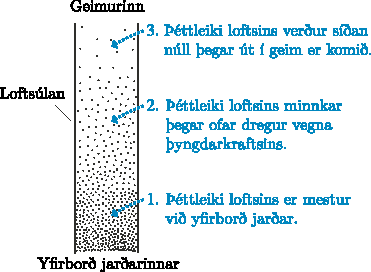
\includegraphics{figures/loftsulan.pdf}
    \caption{Skýringarmynd af loftsúlunni sem sýnir hvernig að þéttleiki loftsins minnkar þegar ofar dregur. Heildarmassinn sem hvílir ofan á herðum okkur vegna súrefnissameindanna ákvarðar staðalþrýstinginn.}
    \label{fig:loftsula}
\end{figure}

Þetta er reyndar smá misleiðandi því einföld sál gæti haldið að að heildarkrafturinn sem verkar á herðar okkar, ef herðar okkar hafa yfirborðsflatarmál $A = \SI{4.0e-2}{m^2}$, væri gefinn með:
\begin{align*}
    F = P_0 A = \SI{1.013e5}{Pa} \cdot \SI{4.0e-2}{m^2} = \SI{4000}{N}.
\end{align*}
En það myndi þá samsvara því að massi $m = \frac{F}{g} = \SI{410}{kg}$ væri lagður ofan á herðar okkar - sem getur ekki staðist! Hvað er að gerast? Það sem gleymist oft í þrýstingsumræðunni er að það er ekki þrýstingurinn sjálfur sem skiptir máli heldur þrýstingsbreytingin. Í þessu tilviki þrýstingsbreytingin yfir og undir herðunum á okkur (reyndar er þrýstingurinn meiri við neðra borð axla okkar svo að heildakrafturinn sem við finnum fyrir vegna þrýstingsins er upp en ekki niður!).


\newpage

\section{Lögmál Pascals}

\begin{minipage}{\linewidth}
\begin{wrapfigure}{r}{2.3in}
    \centering
    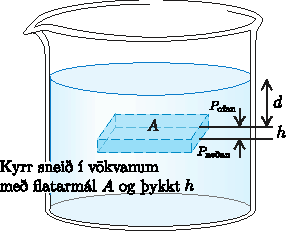
\includegraphics{figures/thykkt.pdf}
    \caption{Kyrr sneið í vökvanum af þykkt $h$ á dýpi $d$ sem hefur þverskurðarflatarmál $A$.}
    \label{fig:dummythick}
\end{wrapfigure}

Skoðum vökva með eðlismassa $\rho_{\text{vökvi}}$. Við gerum ráð fyrir að vökvinn sé um það bil kyrr. Skoðum lárétta sneið af vökvanum sem hefur þverskurðarflatarmáli $A$ og hæð $h$. Látum efri brún kassans sem við skoðum vera við dýpt $d$ en neðri brúnina vera við dýpt $d+h$. Þá er þrýstingurinn á efra borð sneiðarinnar vegna loftsúlunnar og vökvans sem liggur fyrir ofan þverskurðarflatarmálið fenginn með:
\begin{align*}
    P_{\text{ofan}} = P_0 + \frac{\rho_{\text{vökvi}}gdA}{A} = P_0 + \rho_{\text{vökvi}}gd.
\end{align*}
Eins er þrýstingurinn á neðra borð sneiðarinnar gefið með:
\begin{align*}
    P_{\text{neðan}} = P_0 + \frac{\rho_{\text{vökvi}}g(d+h)A}{A} = P_0 + \rho_{\text{vökvi}}g(d+h).
\end{align*}
Þar sem að dýptin var að aukast um $h$. En þar með sjáum við að þrýstingsbreytingin er gefin með:
\begin{align*}
    \Delta P = P_{\text{neðan}} - P_{\text{ofan}} = \left( P_0 + \rho_{\text{vökvi}}g(d+h) \right) -  \left( P_0 + \rho_{\text{vökvi}}gd \right) = \rho_{\text{vökvi}}gh = \rho_{\text{vökvi}}g\Delta d.
\end{align*}
Þar sem að $h = \Delta d$ er dýptarbreytingin í vökvanum. Við sjáum að þrýstingurinn eykst með vaxandi dýpt.

Við höfum þar með sýnt að:

\end{minipage}

\begin{tcolorbox}
\begin{theorem}
\textbf{(Lögmál Pascals)} Lítum á vökva með eðlismassa $\rho_{\text{vökvi}}$. Látum $P_1$ tákna þrýsting vökvans á dýpi $d_1$ og látum $P_2$ tákna þrýsting vökvans á dýpi $d_2$. Þá gildir að þrýstingsbreytingin er gefin með:
\begin{align*}
    \Delta P = \rho_{\text{vökvi}}g\Delta d.
\end{align*}
\end{theorem}
\end{tcolorbox}

Í raun höfum við sýnt mun almennari niðurstöðu heldur en lögmál Pascals hér að ofan. Við höfum sýnt að þrýstingurinn $P$ við dýpið $d$ í vökva með eðlismassa $\rho_{\text{vökvi}}$ er gefinn með:
\begin{align*}
    P = P_0 + \rho_{\text{vökvi}} g d
\end{align*}
þar sem $P_0$ táknar staðalloftþrýstinginn. Það sem er merkilegt við þessa framsetningu er að við sjáum að þrýstingurinn helst fastur alls staðar við sama dýpi í vökvanum!

\section{Lögmál Arkímedesar}



Fræg er sagan af Arkímedesi og krúnu Hiero II Sýrakúsukonungs. Hiero hafði fengið gullsmið nokkurn til þess að smíða kórónu handa sér. En fúskarinn blandaði silfri í blönduna og hélt þannig eftir hluta gullsins. Útaf undarlegri lögun kórónunnar reyndist erfitt að mæla rúmmál hennar (og þar með eðlismassa hennar). Það var ekki fyrr en Arkímedes uppgötvaði sniðuga leið til þess að mæla rúmmál óreglulegra hluta með því að sökkva þeim í vatn sem það komst upp um svikahrappinn. Sagan segir að Arkímedes hafi eftir uppgötvunina hlaupið nakinn um stræti Sýrakúsu og öskrað: \iduck{Eureka!\hspace{0.0001cm}} sem á forngrísku merkir \iduck{Ég hef fundið}. Í daglegu tali þá er lögmál Arkímedesar oftast sett fram með eftirfarandi hætti: \iduck{Sérhver hlutur sem sökkt er að hluta til eða alveg í vökva léttist um það sem nemur þyngd þess vökva sem hann ryður frá sér.} En formlega höfum við að:

\begin{tcolorbox}
\begin{theorem}
\textbf{(Lögmál Arkímedesar)} Lítum á hlut með eðlismassa $\rho_{\text{hlutur}}$ og rúmmál $V_{\text{hlutur}}$ sem sökkt er í vökva með eðlismassa $\rho_{\text{vökvi}}$ sem umlykur hlutinn. Þá verkar á hlutinn uppdrifskraftur, $F_{\text{uppdrif}}$, vegna þrýstingsmunarins, sem er gefinn með:
\begin{align*}
    F_{\text{uppdrif}} = \rho_{\text{vökvi}}V_{\text{hlutur}}g.
\end{align*}
\end{theorem}
\end{tcolorbox}

\begin{minipage}{\linewidth}
\begin{wrapfigure}{r}{2.3in}
    \centering
    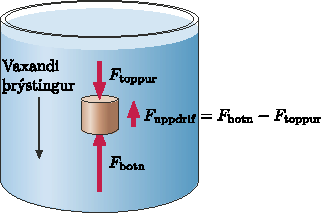
\includegraphics{figures/uppdrif.pdf}
    \caption{Uppdrifskrafturinn orsakast af þrýstingsmuninum við efra og neðra borð hlutarins.}
    \label{fig:uppdrif}
\end{wrapfigure}

\textbf{Útleiðsla:} Við skulum leiða niðurstöðuna út fyrir kassa með eðlismassa $\rho_{\text{hlutur}}$ og rúmmál $V_{\text{hlutur}} = Ah$ þar sem $A$ er þverskurðarflatarmál kassans og $h$ er hæð hans. Hugsum okkur nú að við dýfum kassanum í vökva með eðlismassa $\rho_{\text{vökvi}}$. Þá er ljóst að á neðra borð kassans verkar meiri kraftur vegna þrýstingsins heldur en á efra borðið þar sem að þrýstingurinn er meiri neðar í vökvanum. Látum $y_{\text{botn}}$ tákna hæðina sem botn kassans er við og látum $y_{\text{toppur}}$ tákna hæðina sem toppur kassans er við. Þá höfum við að:
\begin{align*}
    F_{\text{uppdrif}} &= F_{\text{botn}} - F_{\text{toppur}} \\
    &= AP_{\text{botn}} - AP_{\text{toppur}} \\
    &= A \Delta P \\
    &= A \rho_{\text{vökvi}}g\Delta y \\
    &= \rho_{\text{vökvi}}V_{\text{hlutur}}g. \hspace{2cm} \qed
\end{align*}
\end{minipage}


\section{Inngangur að vökvaaflfræði}

\begin{tcolorbox}
\begin{definition}
Við segjum að streymi vökva sé
\begin{enumerate}[label = \textbf{(\roman*)}]
    \item \textbf{lagstreymt} ef hraði vökvans er lítill og stefna hans breytist lítið sem fall af staðsetningu.
    \item \textbf{iðustreymt} ef hraði vökvans er mikill og stefna hans breytist ört sem fall af staðsetningu.
\end{enumerate}
\end{definition}
\end{tcolorbox}




\begin{tcolorbox}
\begin{definition}
Við segjum að vökvi sé \textbf{ósamþjappanlegur} ef að eðlismassi vökvans, $\rho(\Vec{r},t) = \rho$, er fasti sem fall af bæði staðsetningu og tíma.
\end{definition}
\end{tcolorbox}

Í alvörunni eru ekki til nein ósamþjappanleg flæðiefni. Þetta er hinsvegar mjög góð nálgun í flestum þeim tilvikum sem við munum skoða.

\begin{tcolorbox}
\begin{definition}
Við segjum að vökvi sé \textbf{seigjulaus} ef að það er enginn núningur á milli sameinda vökvans. 
\end{definition}
\end{tcolorbox}

Aftur, þá er tæknilega séð ekki til neitt seigjulaust flæðiefni. Hinsvegar þá er ofurflæðandi helíum svo gott sem seigjulaust við $\SI{2}{K}$.

\begin{tcolorbox}
\begin{definition}
Vökvi er sagður vera \textbf{kjörvökvi} ef hann er lagstreyminn, ósamþjappanlegur og seigjulaus.
\end{definition}
\end{tcolorbox}



\section{Samfeldnilögmálið}

\begin{tcolorbox}
\begin{definition}
Lítum á vökva sem sem streymir hornrétt í gegnum yfirborð $A$ með hraða $v$. \textbf{Flæði} vökvans, er táknað með $\Phi$, og skilgreint þannig að:
 \begin{align*}
     \Phi = Av.
 \end{align*}
\end{definition}
\end{tcolorbox}

Það er oftast þægilegast að ímynda sér vatnsflæði í gegnum vatnsrör sem hefur breytilega þykkt og hæð þegar maður leiðir út hinar ýmsu niðurstöður í vökvafræði. Hinsvegar, þá gilda niðurstöðurnar í mun almennara samhengi.

\begin{tcolorbox}
\begin{theorem}
Flæði, $\Phi$, í ósamþjappanelgum vökvum, er varðveitt. M.ö.o.~höfum við að:
\begin{align*}
    A_1 v_1 = A_2 v_2
\end{align*}
\end{theorem}
\end{tcolorbox}

\textbf{Útleiðsla:} Skoðum lítinn tíma $dt$. Þá mun vatnið hafa streymt inn um pípuna um vegalengd $\Delta x_1 = v_1 dt$ en á út um pípuna um vegalengd $\Delta x_2 = v_2 dt$. En þá er massi vatnsins sem kemur inn í pípuna gefið með
\begin{align*}
    m_{\text{inn}} = \rho_{\text{vökvi}} A_1 \Delta x_1 = \rho_{\text{vökvi}} A_1 v_1 dt.
\end{align*}
Það sem streymir út er síðan gefið með:
\begin{align*}
    m_{\text{út}} = \rho_{\text{vökvi}} A_2 \Delta x_2 = \rho_{\text{vökvi}} A_2 v_2 dt.
\end{align*}
En massi vatnsins sem fer inn verður að vera jafn massa vatnsins sem fer út svo við höfum að:
\begin{align*}
    m_{\text{inn}} = m_{\text{út}} \implies \rho_{\text{vökvi}} A_1 v_1 dt =  \rho_{\text{vökvi}} A_2 v_2 dt \implies A_1 v_1 = A_2 v_2.
\end{align*}
Sem sýnir að flæði vökvans, $\Phi$, er varðveitt stærð.

\qed



\section{Lögmál Bernoullis}

\begin{tcolorbox}
\begin{theorem}
\textbf{(Lögmál Bernoullis)} Lítum á sneið í kjörvökva þar sem að þrýstingurinn er $P_1$ og vökvinn streymir í gegnum yfirborð $A_1$ með hraða $v_1$. Lítum á aðra sneið í vökvanum þar sem að þrýstingurinn er $P_2$ og vökvinn streymir í gegnum yfirborð $A_2$ með hraða $v_2$. Þá er stærðin $ P + \rho g h + \frac{1}{2}\rho v^2$ varðveitt, eða með öðrum orðum:
\begin{align*}
    P_1 + \rho g h_1 + \frac{1}{2}\rho v_1^2 =  P_2 + \rho g h_2 + \frac{1}{2}\rho v_2^2
\end{align*}
\end{theorem}
\end{tcolorbox}

\begin{minipage}{\linewidth}
\begin{wrapfigure}{r}{2.3in}
    \vspace{-1cm}
    \centering
    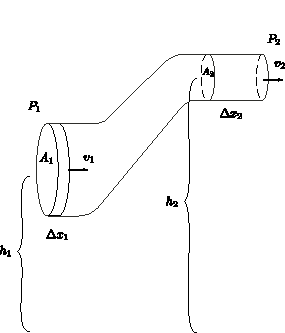
\includegraphics[scale = 1.2]{figures/bernoulli.pdf}
    \label{fig:bern}
\end{wrapfigure}

\textbf{Útleiðsla:} Skoðum flæði vökvans við lítinn tíma $dt$. Þá hefur vökvinn færst inn í rörið um vegalengd $\Delta x_1 = v_1 dt$ og út úr rörinu um vegalengd $\Delta x_2 = v_2 dt$. Við athugum að samkvæmt samfelldnilögmálinu þá er rúmmál vökvans sem yfirgefur rörið jafnt, þ.e.
\begin{align*}
     A_1 \Delta x_1 = A_1 v_1 dt = A_2 v_2 dt = A_2 \Delta x_2.
\end{align*}
Þrýstingurinn í rörinu þegar vatnið er að streyma inn í pípuna vinnur þá vinnu á vatninu sem jafngildir:
\begin{align*}
    W_1 = F_1 \Delta x_1 = P_1 A_1 \Delta x_1, \hspace{1cm} W_2 = -F_2 \Delta x_2 = -P_2 A_2 \Delta x_2.
\end{align*}
Þar sem að $\Vec{F}_2$ og $\Delta \Vec{x}_2$ eru gagnstefna. En þá gefur vinnulögmálið að:
\end{minipage}
\begin{align*}
    W_{\text{heild}} = \Delta K &\implies W_1 + W_2 + W_{g} = \Delta K \\
    &\implies P_1 A_1 \Delta x_1 - P_2A_2 \Delta x_2 - m_1g \Delta h = \frac{1}{2}m_2 v_2^2 - \frac{1}{2}m_1v_1^2 \\
    &\implies P_1 A_1 \Delta x_1 - P_2A_2 \Delta x_2 - \rho A_1 \Delta x_1 g \Delta h = \frac{1}{2} \rho A_2 \Delta x_2 v_2^2 - \frac{1}{2} \rho A_1 \Delta x_1 v_1^2 \\
    &\implies P_1 - P_2 - \rho g\Delta h = \frac{1}{2}\rho v_2^2 - \frac{1}{2}\rho v_1^2 \\
    &\implies P_1 + \rho g h_1 + \frac{1}{2}\rho v_1^2 = P_2 + \rho g h_2 + \frac{1}{2}\rho v_2^2.
\end{align*}
\qed


\newpage

\section{Dæmi}

\begin{enumerate}[label = \textbf{Dæmi \thechapter.\arabic*.}]

\subsection*{Þrýstingur}

\begin{comment}
\item Af hverju er það svona vont þegar fólk stígur ofan á mann í hælaskóm? Venjulegir Crocs skósólar hafa flatarmál $A_1 = \SI{200}{cm^2}$ en hælinn á dæmigerðum hælaskó hefur geisla $r = \SI{50}{mm}$.
\begin{enumerate}[label = \textbf{(\alph*)}]
    \item Hvert er flatarmál hælsins, $A_2$?
    \item Lítum á manneskju með massa $m = \SI{60}{kg}$ sem klæðist Crocs á vinstri fæti og hælaskóm á hægri fæti. Hver er þrýstingur konunnar, $P_1$, niður á jörðina á vinstri fæti og hver er þrýstingur konunnar, $P_2$, niður á jörðina á hægri fæti vegna þyngdar hennar?
\end{enumerate}
\end{comment}

\item \textit{(RK 14.6.)} Hæsti punktur yfirborðs jarðar er Everestfjall, \SI{8850}{m} yfir sjávarmáli, en sá lægsti í Challengergjá í Maríanadjúpálnum í Kyrrahafinu, á \SI{10994}{m} dýpi undir sjávarmáli. Hver er þrýstingurinn á botni Maríanadjúpálsins? (Eðlismassi sjávar er $\rho_{\text{sjór}} = \SI{1030}{kg/m^3}$).

\item \textit{(RK 14.9.)} Eðlismassi vants er $\rho_{\text{vatn}} = \SI{1000}{kg/m^3}$ en eðlismassi olíu er $\rho_{\text{olía}} = \SI{950}{kg/m^3}$. Það þýðir að olía flýtur ofan á vatni. Í stórum vatnstanki hefur olíu verið hellt út í tankinn. Vatnsyfirborðið er í hæð $\SI{120}{cm}$ en olían hefur þykkt $\SI{50}{cm}$. Hver er þrýstingurinn á botni vatnstanksins?

\item \textit{(RK 14.10.)} Kafbátur nokkur hefur glugga með geisla $r = \SI{10}{cm}$ og þykkt $þ = \SI{8.0}{cm}$. Framleiðandi kafbátsins segir að glerið geti þolað heildarkraft $F_{\text{heild}} = \SI{2.0e6}{N}$. Hver er mesta dýpt sem kafbáturinn má kafa ef þrýstingurinn inni í kafbátnum er alltaf $\SI{1}{atm}$.

\item Bergljót Vilbertsdóttir keyrir bílnum sínum fram af bjargi. Þegar bíllinn hefur sokkið niður á $\SI{6.0}{m}$ dýpi reynir Bergljót að opna bílhurðina sem hefur flatarmál $\SI{0.76}{m^2}$. Hversu miklum krafti þarf Bergljót að beita á bílhurðina til þess að opna hana ef þrýstingurinn inni í bílnum er $\SI{1.0}{atm}$?

\vspace{0.5cm}

\begin{minipage}{\linewidth}

\begin{wrapfigure}{r}{1.5in}
\vspace{-0.75cm}
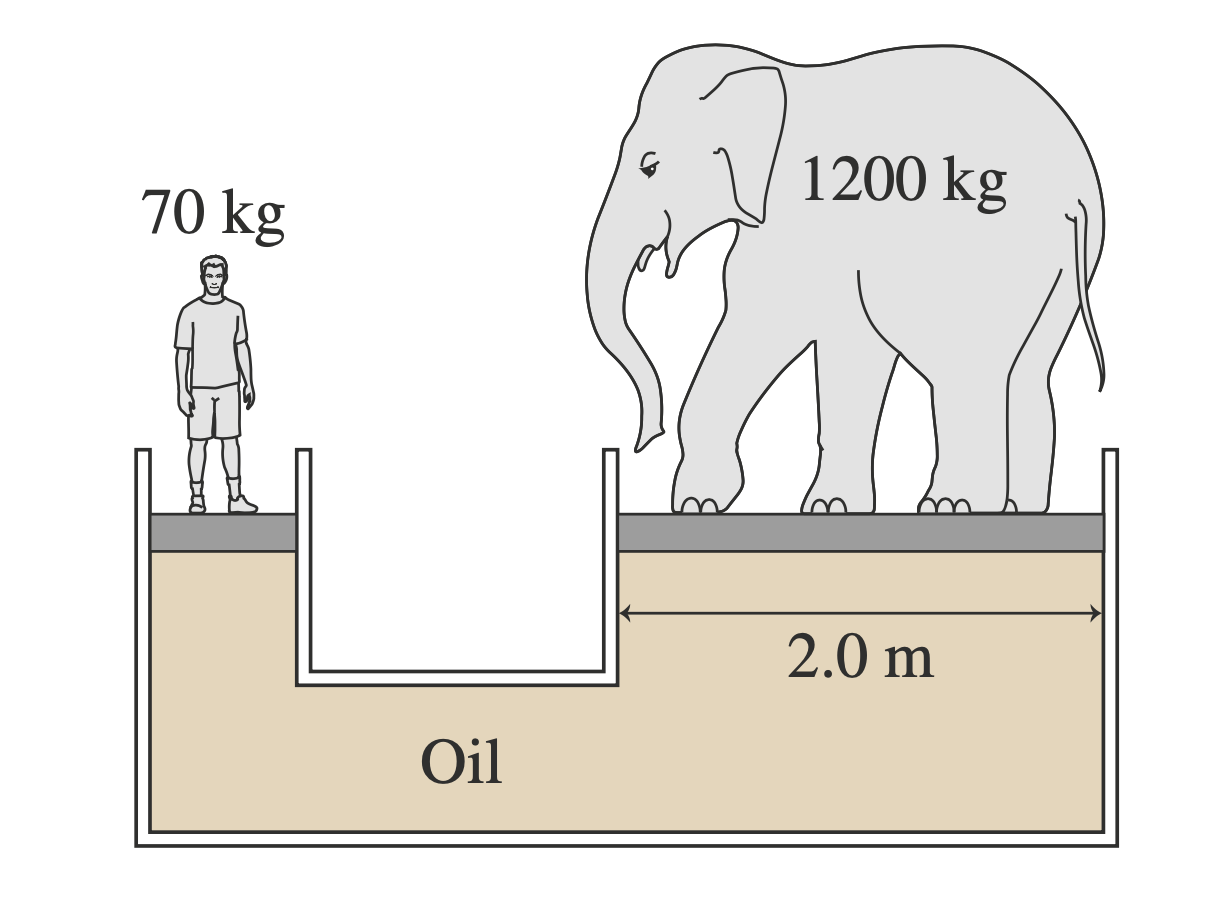
\includegraphics[width=2in]{images/fill.png}
\end{wrapfigure}

\item \textit{(RK 14.42.)} Fíll með massa $M = \SI{1200}{kg}$ stendur ofan á hægri bullunni í vökvalyftu sem hefur geislann $r_2 = \SI{1.0}{m}$. Karið er fyllt með olíu sem hefur eðlismassann $\rho_{\text{olía}} = \SI{950}{kg/m^3}$. Á vinstri bullunni (í sömu hæð og fíllinn) stendur maður með massann $m_1 = \SI{70}{kg}$.

\begin{enumerate}[label = \textbf{(\alph*)}]
    \item Hver er geisli bullunnar sem maðurinn stendur á?
    \item Nú kemur eiginkona mannsins og stígur ofan á bulluna með manninum sínum. Þá sígur vinstri bullan niður um vegalengd $d = \SI{35}{cm}$ en fíllinn helst kyrr í sömu hæð og áður. Hver er massi eiginkonunar?
\end{enumerate}

\end{minipage}

\vspace{0.5cm}

\begin{minipage}{\linewidth}

\begin{wrapfigure}{r}{1in}
\vspace{-0.75cm}
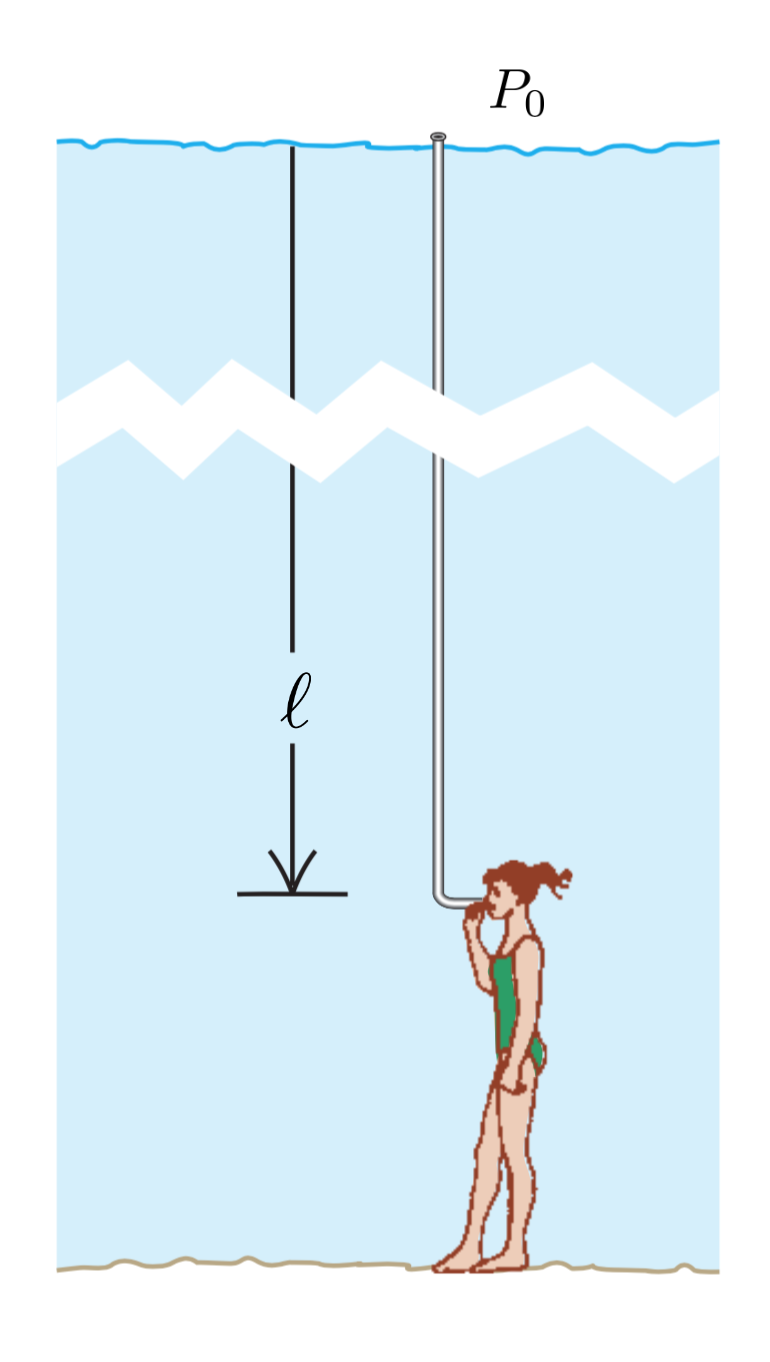
\includegraphics[scale = 0.245]{images/kafa2.png}
\end{wrapfigure}

\item Það er hin prýðilegasta skemmtun að snorkla. Það eru hinsvegar takmarkanir á því hversu djúpt snorklari má kafa. Eftir því sem að dýpið verður meira verður þrýstingsmunurinn meiri. Manneskjan þolir mest $\SI{6000}{Pa}$ þrýstingsmun áður en hún hættir að geta andað. Hver er lengd lengstu snorklunarpípu þannig að snorklari geti andað í gegnum hana?

\subsection*{Lögmál Arkímedesar}

\item \textit{(RK 14.23)} Þegar leirstytta er vegin í lofti sýnir kraftmælirinn $\SI{28.4}{N}$ en þegar styttunni er dýft ofan í vatn þá sýnir kraftmælirinn aðeins $\SI{17.0}{N}$. Hver er eðlismassi leirstyttunnar?

\item \textit{(RK 14.24)} Gegnheil frauðplastkúla með þvermál $\SI{50}{cm}$ og eðlismassa $\SI{150}{kg/m^3}$ flýtur úti á rúmsjó. Hversu stórt hlutfall kúlunnar hvílir undir yfirborði sjávar?

\end{minipage}

\begin{minipage}{\linewidth}

\begin{wrapfigure}{r}{1in}
\vspace{-0.5cm}
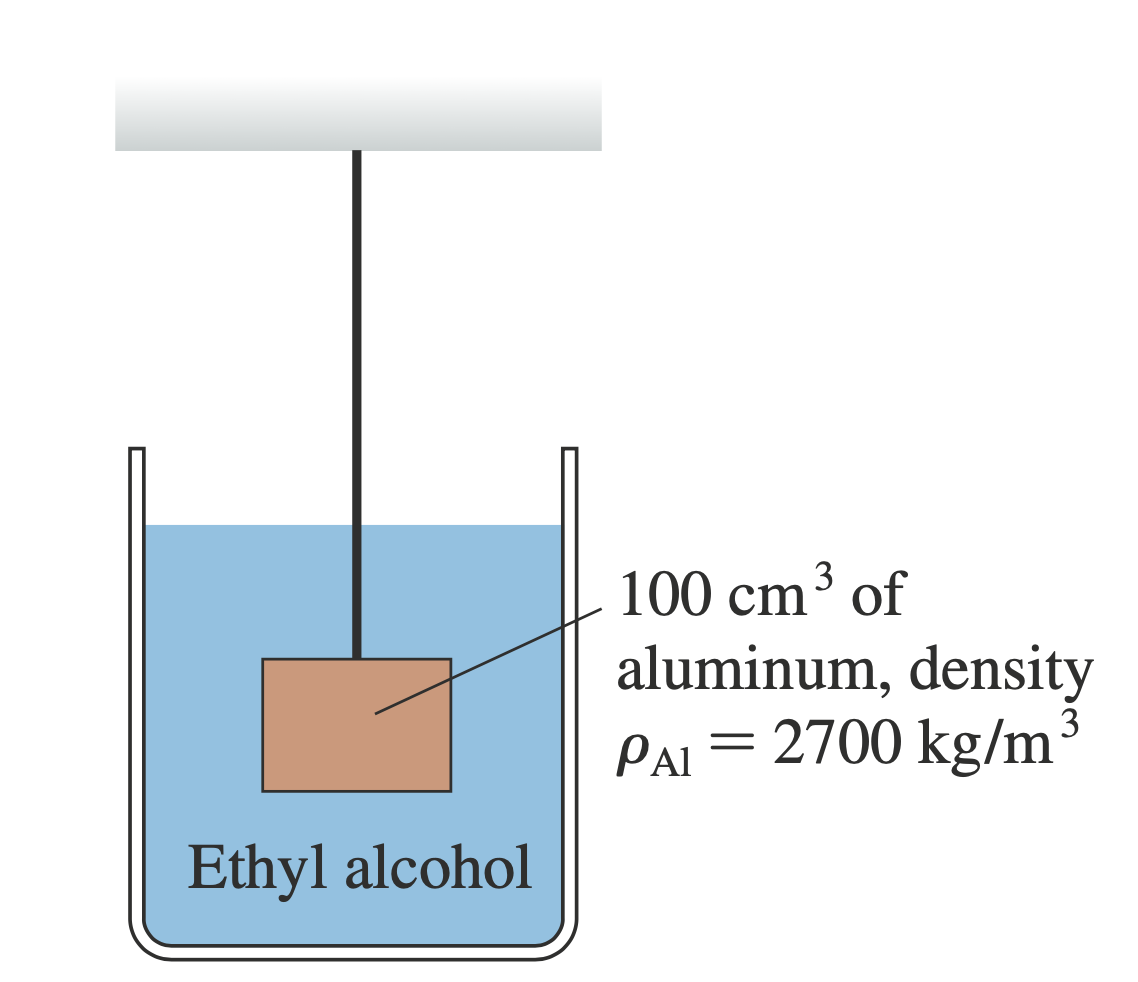
\includegraphics[width=1.5in]{images/alkubb.png}
\end{wrapfigure}

\item Sjór hefur eðlismassa $\rho_{\text{sjór}} = \SI{1027}{kg/m^3}$ og ís hefur eðlismassa $\rho_{\text{ís}} = \SI{920}{kg/m^3}$. Hversu stór hluti af ísjaka stendur upp úr yfirborði sjávar?

\item \textit{(RK 14.21.)} Álkubbur með rúmmál $\SI{100}{cm^3}$ og eðlismassa $\rho_{\text{ál}} = \SI{2700}{kg/m^3}$ hangir á $\SI{5.0}{cm}$ dýpi í íláti sem er fyllt með etanóli ($\rho_{\text{etanól}} = \SI{789}{kg/m^3}$). Kubburinn hangir kyrr í massalausu bandi. Hver er togkrafturinn í bandinu?

\item \textit{(RK 14.71)} Botninn á stálbát (meira eins og stálkassi sem vantar lok) hefur breidd $b = \SI{5.0}{m}$, lengd $\ell = \SI{10}{m}$ og þykkt $d = \SI{2.0}{cm}$. Hliðar bátsins hafa þyktina $þ = \SI{0.50}{cm}$. Eðlismassi stáls er $\rho_{\text{stál}} = \SI{7900}{kg/m^3}$. Hver er minnsta hæðin, $h$, sem að hliðar bátsins þurfa að hafa þannig að hann geti flotið á lygnum sjó?

\end{minipage}

\vspace{2cm}


\begin{minipage}{\linewidth}

\begin{wrapfigure}{r}{1.3in}
\vspace{-1.5cm}
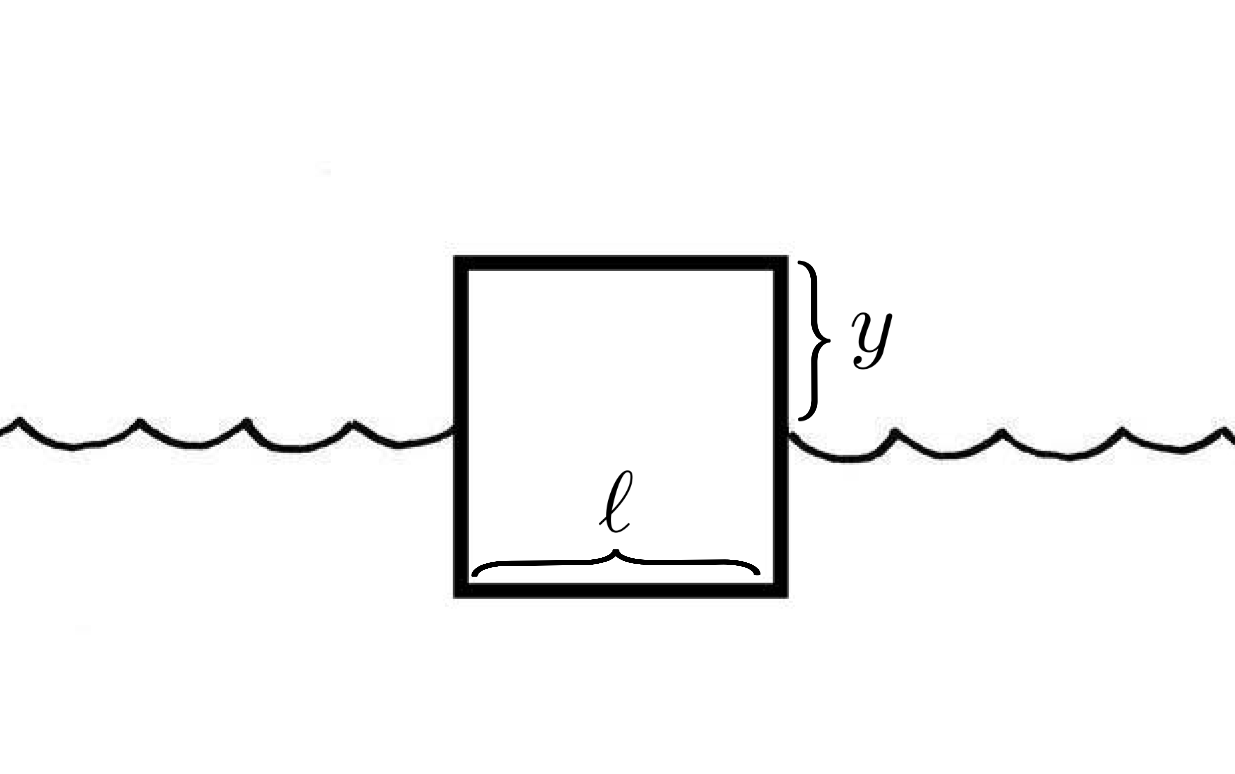
\includegraphics[width=1.8in]{images/kubbursjor.png}
\end{wrapfigure}

\item \textbf{(Vorpróf 2019)} Gegnheill kassi með allar hliðar jafnlangar, $\ell = \SI{0.50}{m}$, og með eðlismassa $\rho_k = \SI{650}{kg/m^3}$ flýtur úti á rúmsjó. Eðlismassi sjávar er $\rho_s = \SI{1027}{kg/m^3}$. Finnið hæð kassans, $y$, sem flýtur fyrir ofan yfirborð sjávar.

\end{minipage}

\vspace{0.4cm}

\begin{minipage}{\linewidth}

\begin{wrapfigure}{r}{1.1in}
\vspace{-1cm}
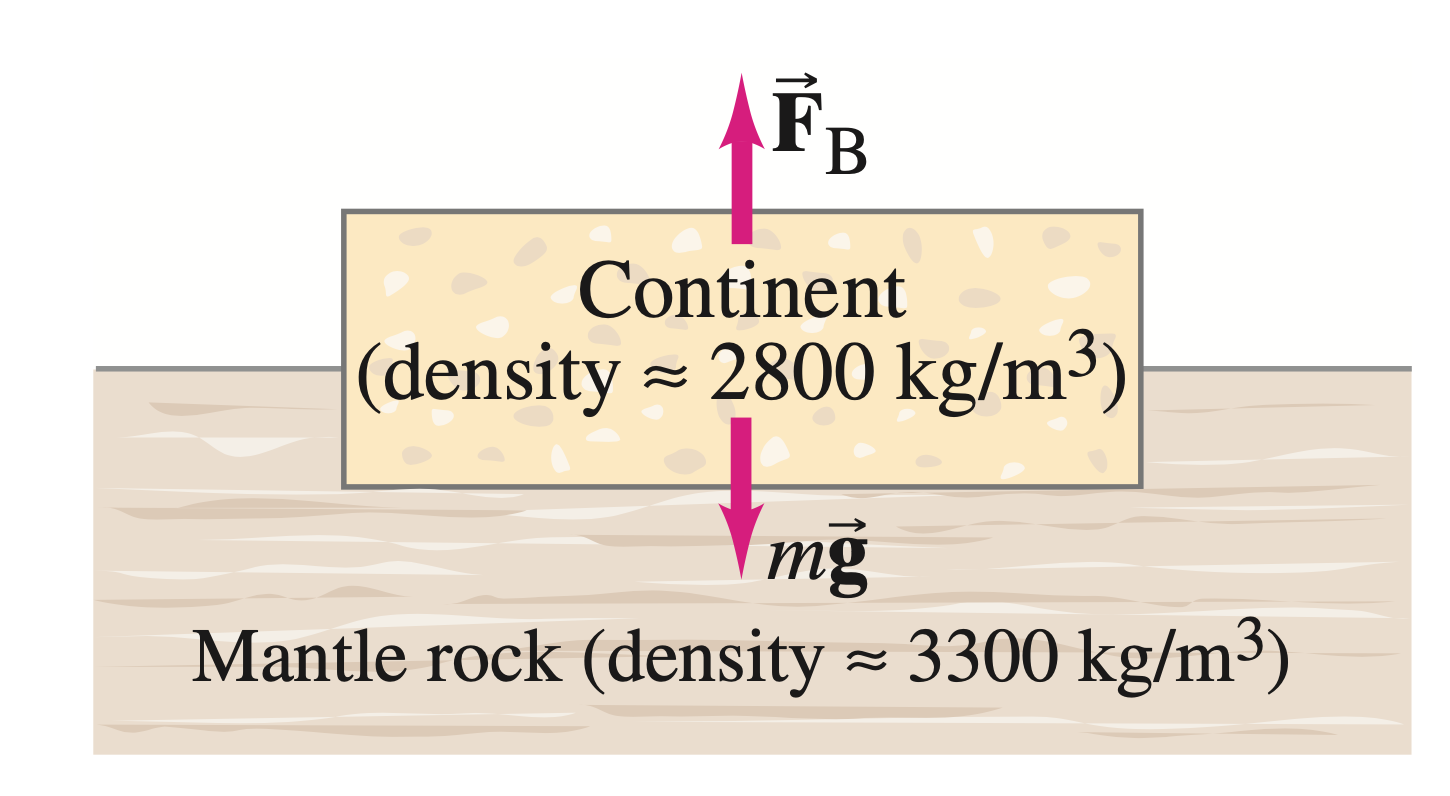
\includegraphics[width=1.5in]{images/jardskorpa.png}
\end{wrapfigure}

\item Einfalt líkan af flekahreyfingum lítur á sem svo að flekarnir samanstandi af rétthyrningslaga kubbum með þykkt $þ = \SI{35}{km}$ og eðlismassa $\rho_{\text{fleki}} = \SI{2800}{kg/m^3}$ sem fljóta á jarðmöttlinum sem er vökvi með eðlismassa $\rho_{\text{möttull}} = \SI{3300}{kg/m^3}$. Hversu stór hluti af hæð jarðskorpunnar flýtur fyrir ofan yfirborð möttulsins?
\end{minipage}



\item \textit{(RK 14.54.)} Gormur með gormstuðul $k = \SI{35}{N/m}$ er festur í annan enda við loftið og í hinn endan við sívalning með massa $m = \SI{1.0}{kg}$,  geisla $r = \SI{2.5}{cm}$ og hæð $h = \SI{10}{cm}$. Sívalningnum er haldið þannig að gormurinn sé hvorki strekktur né þjappaður. Íláti með vatni er komið fyrir þannig að neðra borð sívalningsins snertir vatnið. Þegar kerfinu er sleppt úr kyrrstöðu byrjar sívalningurinn að sveiflast um í vatninu þar til að núningurinn við vatnið stöðvar sívalninginn ofan í vatninu við dýpt $d$. Hvert er gildið á dýptinni $d$?

\begin{minipage}{\linewidth}

\begin{wrapfigure}{r}{1.1in}
\vspace{-1cm}
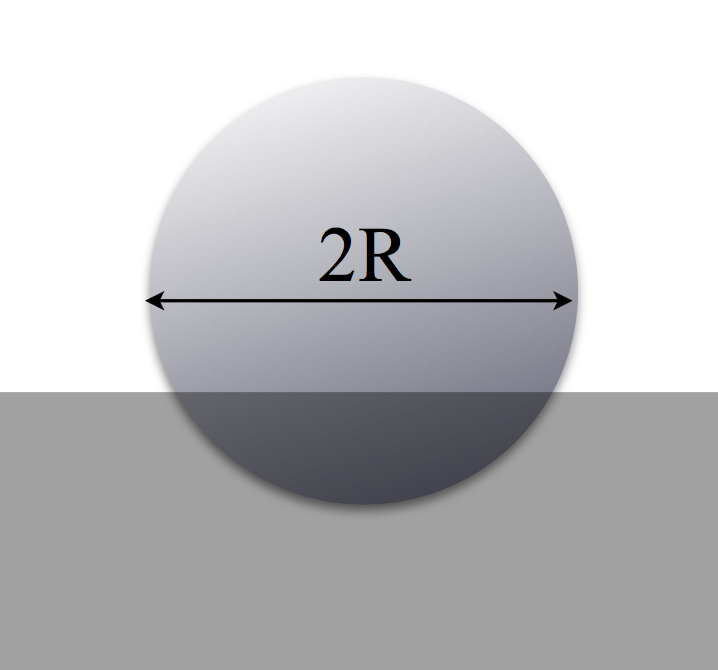
\includegraphics[width=1.5in]{images/kula.png}
\end{wrapfigure}

\item Plastbolti með geisla $R = \SI{0.19}{m}$ flýtur á vatni þannig að $24 \%$ af rúmmáli boltans eru fyrir neðan vatnsborðið.
\end{minipage}
\begin{enumerate}[label = \textbf{(\alph*)}]
    \item Hve miklum krafti þarf að beita á boltann til þess að halda honum \\ öllum rétt fyrir neðan vatnsborðið?
    
    \item Hver verður hröðun boltans einmitt þegar honum er sleppt?
\end{enumerate}


\subsection*{Samfelldnilögmálið og Lögmál Bernoullis}

\item \textit{(RK 14.26.)} Garðslanga nokkur hefur þvermál $þ = \SI{19}{mm}$. Hver er hraði vatnsins þegar það yfirgefur slönguna ef það tekur $\SI{8}{mín}$ að fylla uppblásna $\SI{600}{L}$ barnavaðlaug með garðslöngunni.


\begin{minipage}{\linewidth}
\begin{wrapfigure}{r}{1.3in}
\vspace{-0.5cm}
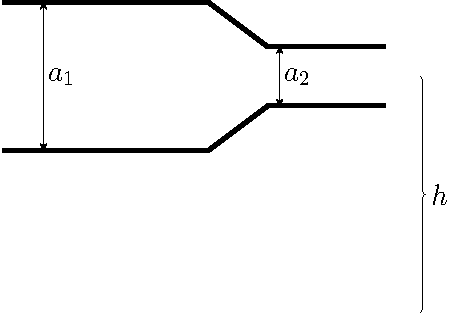
\includegraphics[scale=0.6]{images/pipe_test.pdf}
\end{wrapfigure}

\item \textbf{(Vorpróf 2018)} Vatn streymir í vatnsröri. Vatnsrörið liggur lárétt í hæðinni $h = \SI{1.2}{m}$ og fer úr því að hafa þvermál $a_1 = \SI{4.5}{cm}$ niður í að hafa þvermál $a_2=\SI{1.4}{cm}$ eins og sjá má á mynd. Hraði vatnsins í breiðari endanum er $v_1 = \SI{0.40}{m/s}$.
\begin{enumerate}[label = \textbf{(\alph*)}]
    \item Hver er hraði vatnsins, $v_2$, í mjórri enda vatnsrörsins?
    \item Hvert er flæði vatnsins í hvorum hluta fyrir sig?
    \item Hver er þrýstingsmunurinn á milli breiðari og mjórri enda vatnsrörsins?
\end{enumerate}
\end{minipage}


\begin{minipage}{\linewidth}
\begin{wrapfigure}{r}{1.4in}
\vspace{-0.5cm}
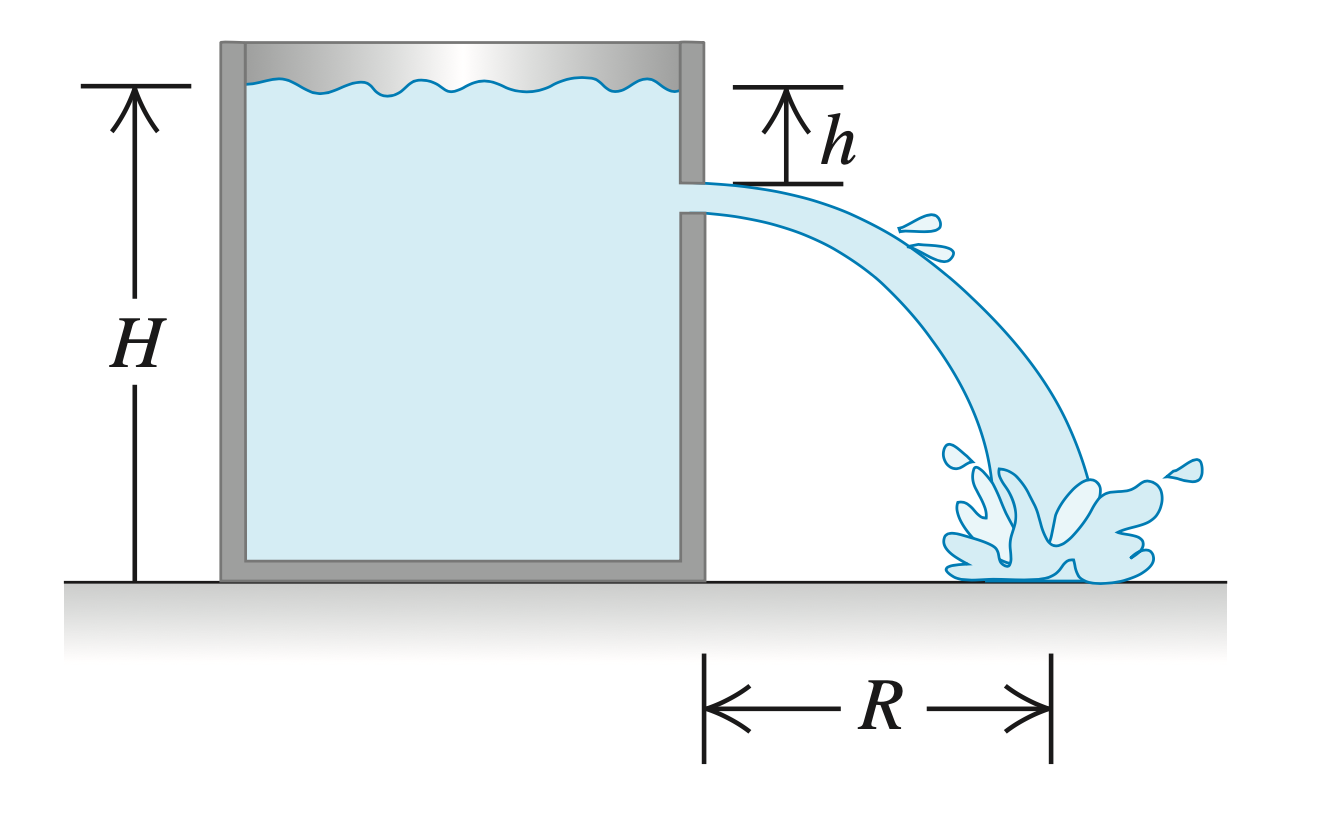
\includegraphics[width = 1.8in]{images/vatnstankur.png}
\end{wrapfigure}

\item Vatnstankar Perlunnar eru sívalningar með geisla $r = \SI{12}{m}$ og hæð $H = \SI{10}{m}$. 
\begin{enumerate}[label = \textbf{(\alph*)}]
    \item Hversu margir lítrar af vatni komast fyrir í vatnstönkunum? Hver er þrýstingurinn á botni vatnstankanna?
    \item Hugsum okkur nú að skemmdarvargar skeri hringlaga gat á vatnstankinn með þvermál $\text{þ} = \SI{3.0}{cm}$ í fjarlægð $h = \SI{2.5}{m}$ frá toppi tanksins. Hver verður hraði vatnsins rétt eftir að gatið hefur verið skorið þegar það spýtist út úr gatinu? Hvert verður flæði þess?  Hvar lendir vatnið?
\end{enumerate}
\end{minipage}

\item Flugvél hefur massa $\SI{1.7e6}{kg}$ og loftið við neðra borð vængsins hefur hraða $\SI{95}{m/s}$. Þverskurðarflatarmál vænganna er $\SI{1200}{m^2}$. Hversu hratt þarf loftið við efra borð vængsins að ferðast til þess að flugvélin haldist í loftinu án þess að hrapa?

\begin{minipage}{\linewidth}
\begin{wrapfigure}{r}{1in}
\vspace{-0.5cm}
\hspace{0.5cm}
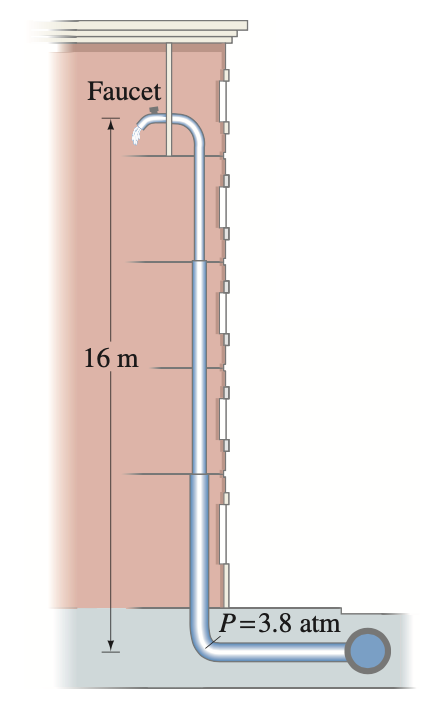
\includegraphics[width = 1in]{images/building.png}
\end{wrapfigure}

\item Vatn við þrýsting $\SI{3.8}{atm}$ streymir inn með hraðanum $\SI{0.78}{m/s}$ í gegnum rör með geisla $\SI{2.5}{cm}$ í kjallaranum á skrifstofubyggingu Lalla lögfræðings. Lalli ætlar að fá sér ískalt og svalandi vatnsglas á efstu hæðinni $\SI{16}{m}$ ofar svo hann kveikir á krananum. Þar er geisli rörsins búinn að minnka niður í $\SI{1.4}{cm}$. Finnið flæði vökvans og þrýstinginn í vatnshananum á efstu hæðinni.

\end{minipage}


\end{enumerate}

\newpage

\section*{Svör}

\begin{enumerate*}[label = \vspace{0.15cm} \textbf{(\arabic*)}]
  \item $P = \SI{1.11e8}{Pa} = \SI{1100}{atm}$. \item $P = \SI{1.18e5}{Pa} = \SI{1.16}{atm}$.
  \item $d = \SI{6290}{m}$.
  \item $F = \SI{45000}{N}$.
  \item $r_1 = \SI{0.24}{m}$, $m_2 = \SI{59}{kg}$.
  \item $h = \SI{0.61}{m}$.
  \item $\rho_{\text{hlutur}} = \SI{2500}{kg/m^3}$.
  \item $p = \SI{15}{\%}$.
  \item $1-p = \SI{10.4}{\%}$.
  \item $T = \SI{1.88}{N}$.
  \item $h = \SI{15.7}{cm}$.
  \item $y = \SI{0.18}{m}$.
  \item $y = \SI{5.3}{km}$.
  \item $x = \SI{2.71}{cm}$.
  \item $\rho_{\text{hlutur}} = \SI{240}{kg/m^3}$, $F = \SI{214}{N}$, $a = \SI{31}{m/s^2}$.
  \item $\Phi = \SI{1.25e-3}{m^3/s} = \SI{1.25}{L/s}$, $v = \SI{4.4}{m/s}$.
  \item $v_2 = \SI{4.1}{m/s}$, $\Phi = \SI{6.36e-4}{m^3/s} = \SI{0.64}{L/s}$, $\Delta P = \SI{-8300}{Pa} = \SI{0.082}{atm}$.
  \item $P = \SI{2.0e5}{Pa} = \SI{1.97}{atm}$, $v_2 = \SI{7.0}{m/s}$, $\Phi = \SI{4.95}{L/s}$, $x = \SI{8.6}{m}$.
  \item $v_2 = \SI{180}{m/s}$.
  \item $v_2 = \SI{2.5}{m/s}$, $P_2 = \SI{2.25e5}{Pa} = \SI{2.22}{atm}$.
\end{enumerate*}

\newpage